% !TEX TS-program = xelatex
% !TEX encoding = UTF-8

\documentclass[11pt,a4paper]{article} 
\usepackage[a4paper,margin=0pt,left=0mm]{geometry}
\usepackage[T1]{fontenc} 
\usepackage{times,graphicx}
\usepackage[grid=true,subgridcolor=green!20,	% grid used only in draft mode
                   gridcolor=gray!80, texcoord=true, 
                   gridunit=cm]{eso-pic}
%\defaultfontfeatures{Mapping=tex-text} 
%\usepackage{xunicode} 
%\usepackage{xltxtra} 
%\usepackage{geometry}
\usepackage{times}
\usepackage{xcolor,rotating}
\usepackage{graphicx} 
\makeatletter
\newif\if@debug
\fboxsep0pt
\fboxrule0pt
\@debugfalse
\if@debug
   \def\rulecolor{gray}%
   \fboxsep-0.2pt 
  \fboxrule0.2pt
\else
  \fboxsep0pt
  \fboxrule0pt
\fi
\parskip0pt
\def\includegraphics#1{\expandafter\@gobble{#1}\rule{100pt}{50pt}}
% first block mitteilungen
  \def\A{\fbox{
\includegraphics{img-01}}}
  \def\B{\fbox{
\includegraphics{img-02}}}
  \def\C{\fbox{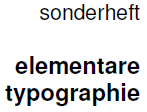
\includegraphics{img-03}}}
  \def\D{\fbox{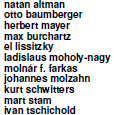
\includegraphics{img-04}}}
  \def\E{\fbox{
\includegraphics{img-05}}}
  \def\offsetXY#1#2#3{\hskip#1\raise#2\vbox{\hbox{#3}}}
  \def\offsetY#1{\vspace*{#1}}
  \def\offsetrule#1#2{ \color{\rulecolor}\rule{#1}{#2}}
\parindent0pt
\begin{document}
\makeatletter
\topskip0pt
\parindent0pt
\newlength\xgrid
\newlength\ygrid
\def\hopx#1{\hspace*{#1\xgrid\relax}}
\def\hopy#1{\vspace*{#1\ygrid\relax}}
\setlength\xgrid{54.15pt} % this is possibly correct
\setlength\ygrid{20mm}   % this not sure does not look right
\def\rulei {{\color{red}\rule{6.5in}{1pc}}}
\def\ruleii {{\color{red}\rule{1pc}{23.5cm}}}
\def\ruleiii{{\color{black}\rule{152pt}{10pt}}}


\def\C{\hspace*{\dimexpr\xgrid-7pt}\turnbox{90}{\fbox{\fontsize{52}{50}\sffamily\bfseries \hspace{9mm} mep progress}}}




\newbox\AAA
\setbox\AAA\hbox{%
{\fontsize{52}{50}\sffamily\bfseries \fbox{\hbox to 6.5in{\hfill city center}}}}


\expandafter\protected@xdef\csname AAA@wd\endcsname{\the\wd\AAA}
%  \the\dp\AAA\\
%  \the\ht\AAA\\

% Mitteilungen
\hopy{2}
\vskip3pt

\hspace*{20pt}\rulei\vskip3pt
\hspace*{20pt}\unhbox\AAA\par

% Vertical red stripe

\hspace*{10mm}\vbox to 23.5cm{\fbox{\hbox to \dimexpr 2\xgrid{\hfill\ruleii}}}%

% add typographie
\vspace*{-10.35cm}\hskip2\xgrid\hskip10mm\C 

\vspace{-7.52cm}
\hopx{4}\hspace{4mm}
\fbox{\parbox{180pt}
                 {\raggedleft
                         \fontsize{28}{20}\sffamily sonderheft
                         \vspace{1cm}

                         \fontsize{31}{36}\sffamily\bfseries 
                      elementare\\
                      typographie}}

\vspace*{1.15in}
\hopx{7.5}
\fbox{\parbox{140pt}
                 {\raggedright \fontsize{13}{14}\sffamily\bfseries 
                       natan altman \\
                       otto baumberger \\
                       herbert mayer \\
                       max burchartz \\
                       el lissitzky \\
                       ladislaus moholy-nagy \\
                       moln\'ar f.~farkas \\
                       jahannes molzahn \\
                       kurt schwitters \\
                       mart stam \\
                       ivan tschichold}}

\def\ccc {\fontsize{12}{10}\sffamily 
                      \quad zeitschrift des bildungsverbandes der
                      deutschen buchdrucker leipzig 
                     \textbullet{} oktoberheft 1925}

\let\div\hbox%
%\vspace*{-25.4cm}
\hopy{-12.6}
\hopx{10}\hspace*{15pt}
 \div{\hbox to 23.5cm{{\turnbox{-90}{\fbox{\div{\ccc\kern 3cm\ruleiii}}}}}}
\end{document}



